\subsection{Creazione di un Nuovo Progetto}
Dopo essersi autenticati è possibile creare un nuovo progetto, la richiesta di questa operazione si avvia tramite la parola chiave "crea progetto", quindi il chatbot avvia la creazione e tramite vari messaggi di botta e risposta chiede tutte le informazioni necessarie:
\begin{itemize}
    \item inserire il codice del progetto (se il codice è libero fa proseguire altrimenti chiede un altro codice);
    \item inserire una descrizione;
    \item inserire cliente;
    \item inserire manager;
    \item inserire area (nel senso di luogo);
    \item inserire data inizio;
    \item inserire data fine;
\end{itemize}
Se si inserisce un formato o una parola non valida chiede di reinserire, infine riepiloga tutti i dati ricevuti e chiede conferma se procedere o se si vuole modificare qualche dato o se si vuole annullare la creazione del progetto.

\subsubsection{Schermate Creazione Progetto}
\begin{figure}[H]
    \centering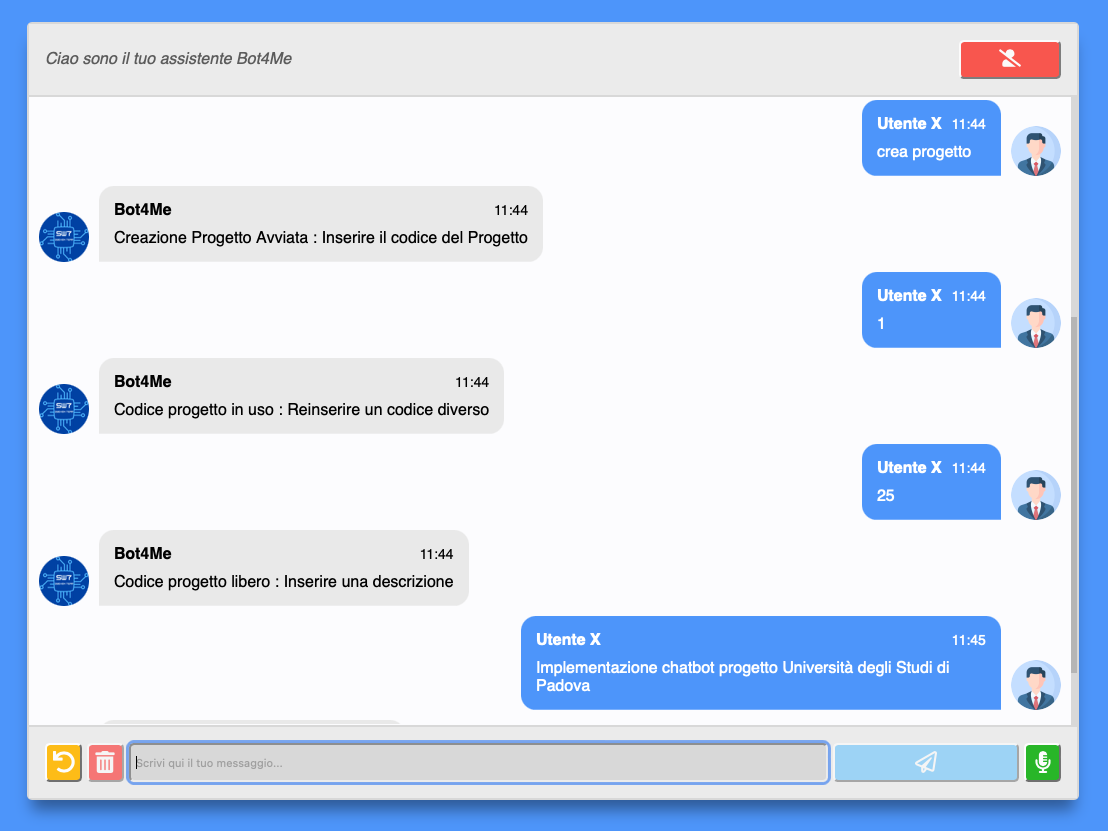
\includegraphics[width=0.8\textwidth, height=0.7\textheight, keepaspectratio]{images/schermata_creazione_progetto_1.png}
    \caption{Schermata Creazione Progetto - Con Inserimento Codice Pre-Esistente}
\end{figure}

\begin{figure}[H]
    \centering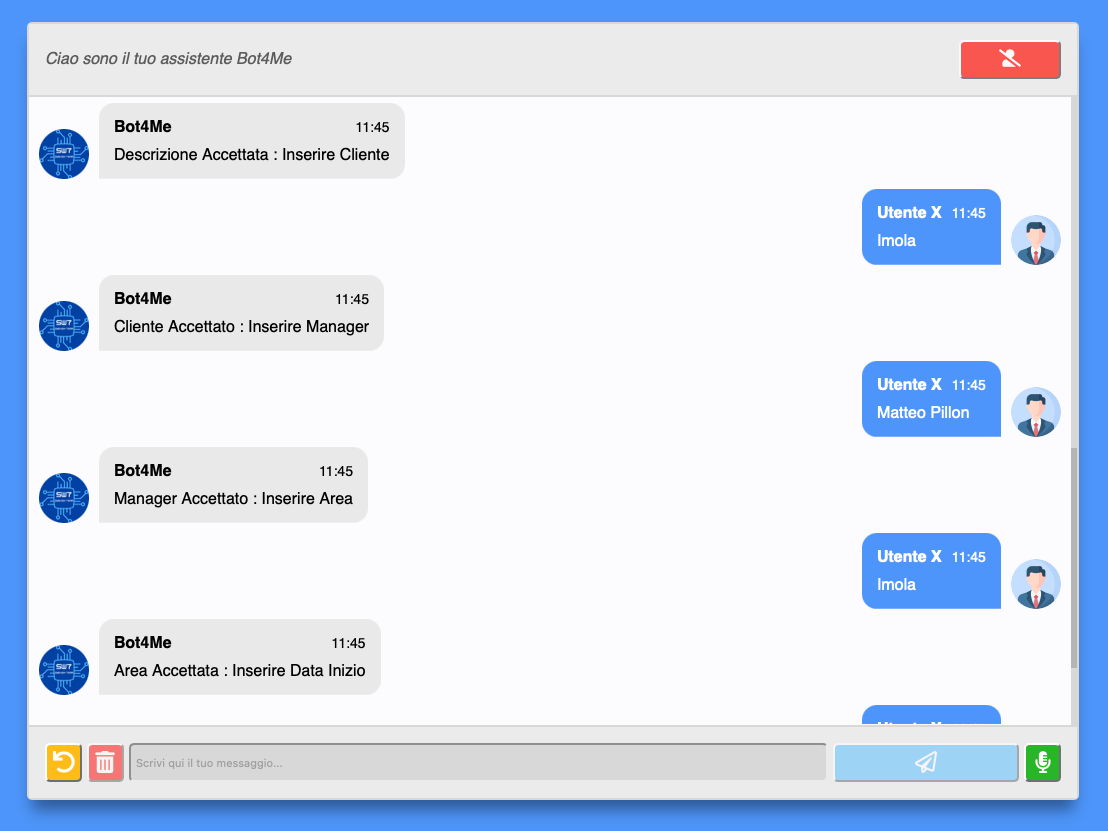
\includegraphics[width=0.8\textwidth, height=0.7\textheight, keepaspectratio]{images/schermata_creazione_progetto_2.png}
    \caption{Schermata Creazione Progetto}
\end{figure}

\begin{figure}[H]
    \centering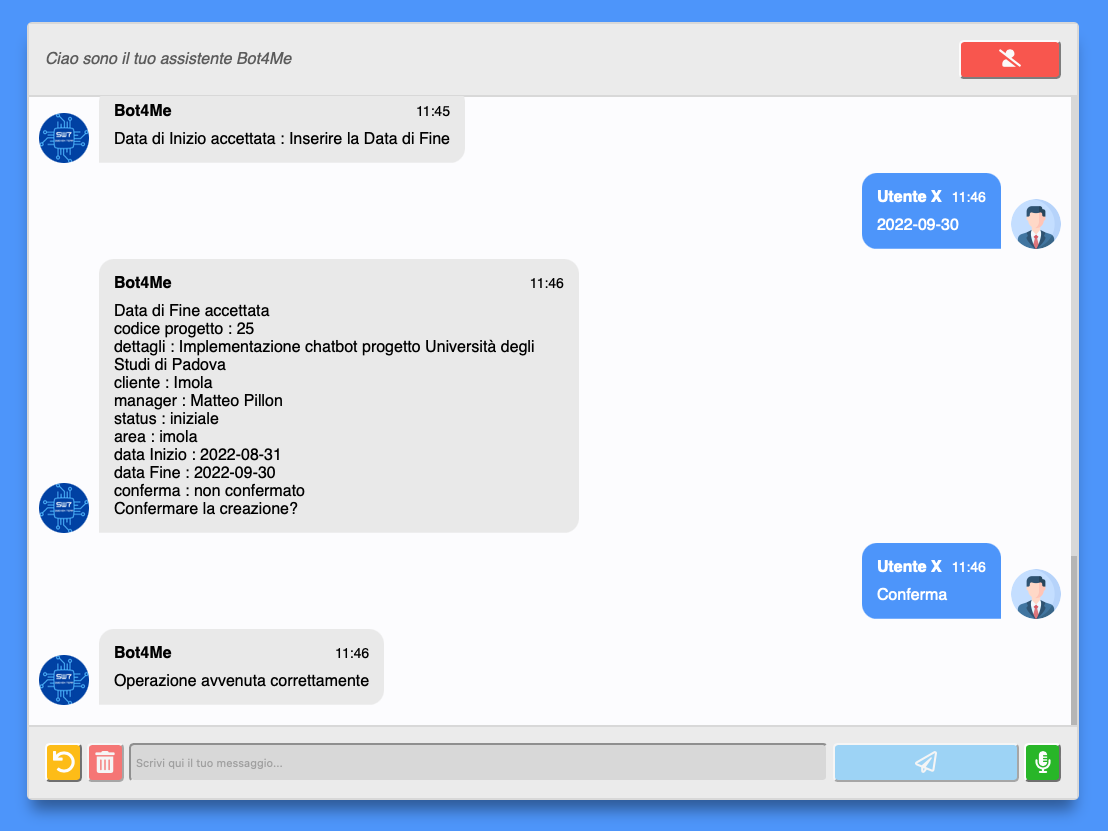
\includegraphics[width=0.8\textwidth, height=0.7\textheight, keepaspectratio]{images/schermata_creazione_progetto_3.png}
    \caption{Schermata Creazione Progetto - Riepilogo e Conferma Operazione}
\end{figure}